The full-system model of the Hyperloop can be decomposed into two main
sub-systems: the passenger pod and tube. At the top level, these systems are
connected to basic cost estimation and notional
mission modules. Below is a tree view of the system.
The appendix includes an eXtended Design Structure Matrix (XDSM) diagram key
which describes how to interpret the following diagrams for the pod, tube, and mission subsystems.

\begin{figure}
\centering
\begin{subfigure}{.5\textwidth}
  \centering
  \includegraphics{../images/tube_and_pod.png}
  \caption{Hierarchial tree}
  \label{fig:tree:tube_and_pod}
\end{subfigure}%
\begin{subfigure}{.5\textwidth}
  \centering
  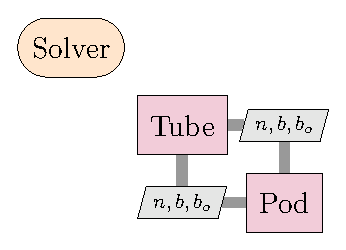
\includegraphics{../images/xdsm/tube_and_pod.pdf}
  \caption{XDSM}
  \label{fig:xdsm:toplevel}
\end{subfigure}
\caption{Top Level System Diagram}
\label{fig:top}
\end{figure}

\begin{figure}
\centering
\begin{subfigure}{.5\textwidth}
  \centering
  \includegraphics{../images/tube.png}
  \caption{Hierarchial tree}
  \label{fig:tree:tube}
\end{subfigure}%
\begin{subfigure}{.5\textwidth}
  \centering
  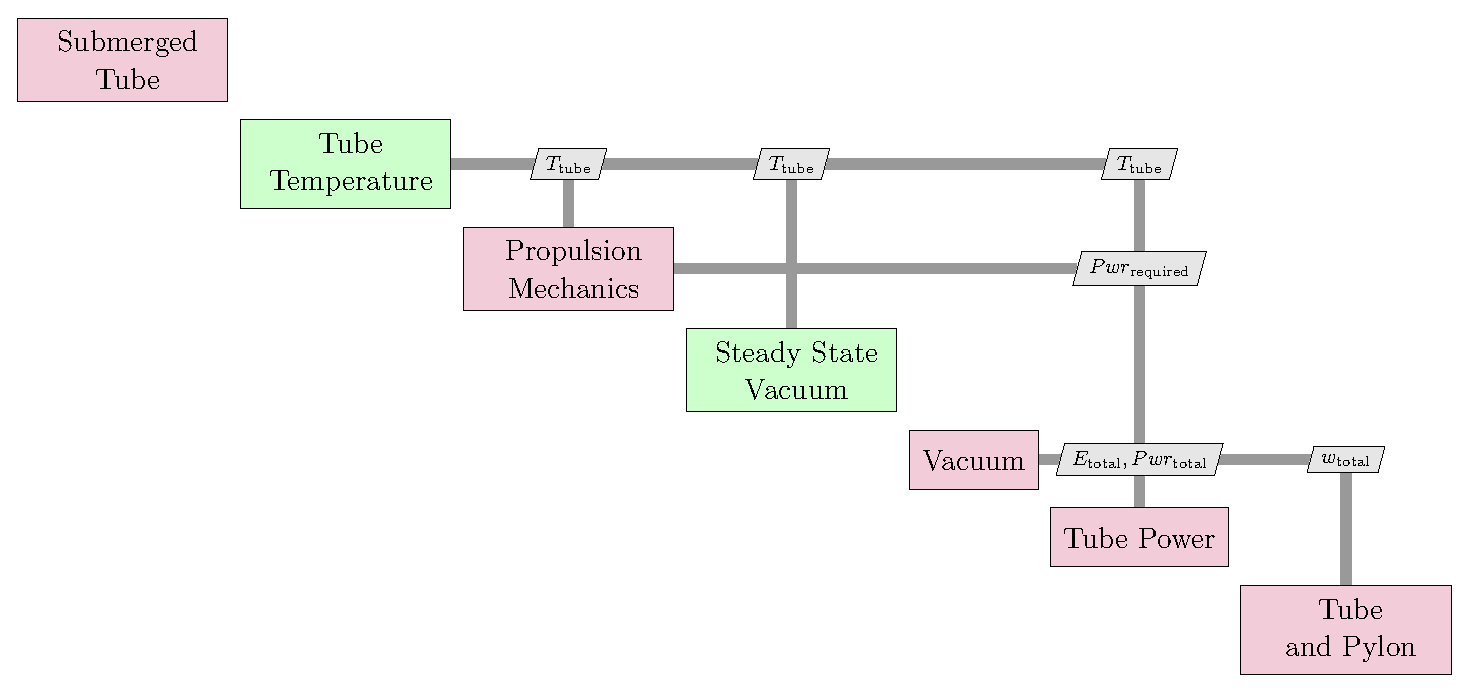
\includegraphics{../images/xdsm/tube.pdf}
  \caption{XDSM}
  \label{fig:xdsm:tube}
\end{subfigure}
\caption{Tube Assembly Diagram}
\label{fig:tube}
\end{figure}

\begin{figure}
\centering
\begin{subfigure}{.5\textwidth}
  \centering
  \includegraphics{../images/pod.png}
  \caption{Hierarchial tree}
  \label{fig:tree:pod}
\end{subfigure}%
\begin{subfigure}{.5\textwidth}
  \centering
  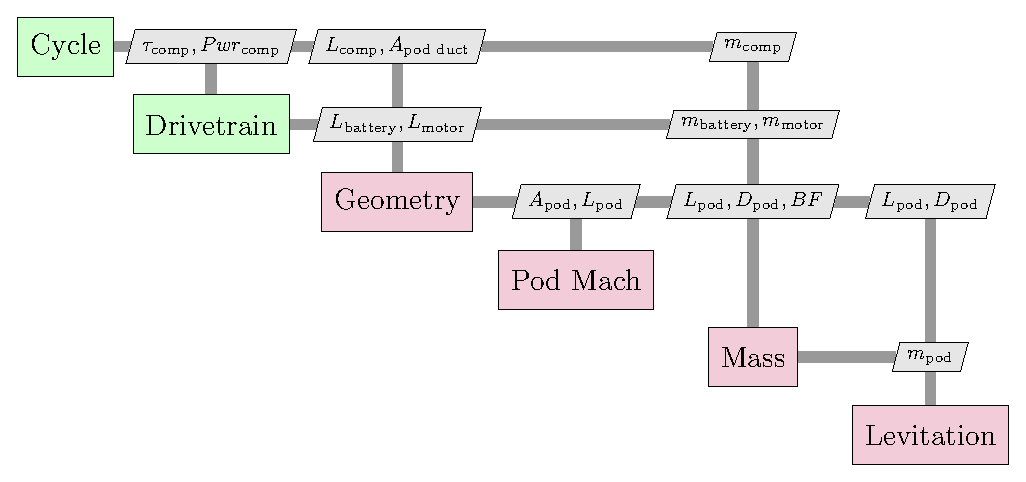
\includegraphics{../images/xdsm/pod.pdf}
  \caption{XDSM}
  \label{fig:xdsm:pod}
\end{subfigure}
\caption{Tube Assembly Diagram}
\label{fig:pod}
\end{figure}

Additional levels of sub-systems were broken down within the pod and tube assemblies.
Solver loops exist at multiple levels within the model, ensuring all design
constraints are satisfied across every sub-component.
The XDSM diagrams indicates design variables that are passed from the output of
upstream components to be used as inputs for downstream components.
Further details can be found in following sections, and the Appendix.

\subsection{Top Level Component Descriptions}
	\subimport{model_overview/}{top_level_comp_descriptions}
\subsection{Pod Level Component Descriptions}
	\subimport{model_overview/}{pod_level_comp_descriptions}
\subsection{Tube Level Component Descriptions}
	\subimport{model_overview/}{tube_level_comp_descriptions}


